% ============================================================================================
% BAB III ANALISIS MASALAH
% Pembagian subbab tidak rigid dan dapat bervariasi. Bab ini minimal berisi analisis kebutuhan
% fungsional dan nonfungsional, analisis berbagai alternatif solusi yang dapat ditawarkan, dan
% metode pemilihan solusi yang diusulkan.
% ============================================================================================
\cleardoublepage
\chapter{ANALISIS MASALAH}
\label{chap:analisis-masalah}
\section{Analisis Kondisi Saat Ini}
\label{sec:kondisi_saat_ini}

Berdasarkan tinjauan terhadap sistem pertiketan elektronik konvensional yang umum digunakan saat ini (seperti pada studi kasus konser musik dan pertandingan olahraga), model proses bisnis yang berjalan masih mengandalkan arsitektur kode QR statis. Sesuai dengan pendekatan analisis sistem informasi menurut \textcite{laudon2020}, kondisi eksisting dimodelkan terlebih dahulu untuk memetakan interaksi antar-entitas dan mengidentifikasi titik-titik kegagalan sistem. Model konseptual dari sistem yang berjalan, beserta titik-titik kerentanan yang teridentifikasi dalam alur distribusi dan validasi tiket, digambarkan pada Gambar \ref{fig:current_system_flow}.

\begin{figure}[htbp]
    \centering
    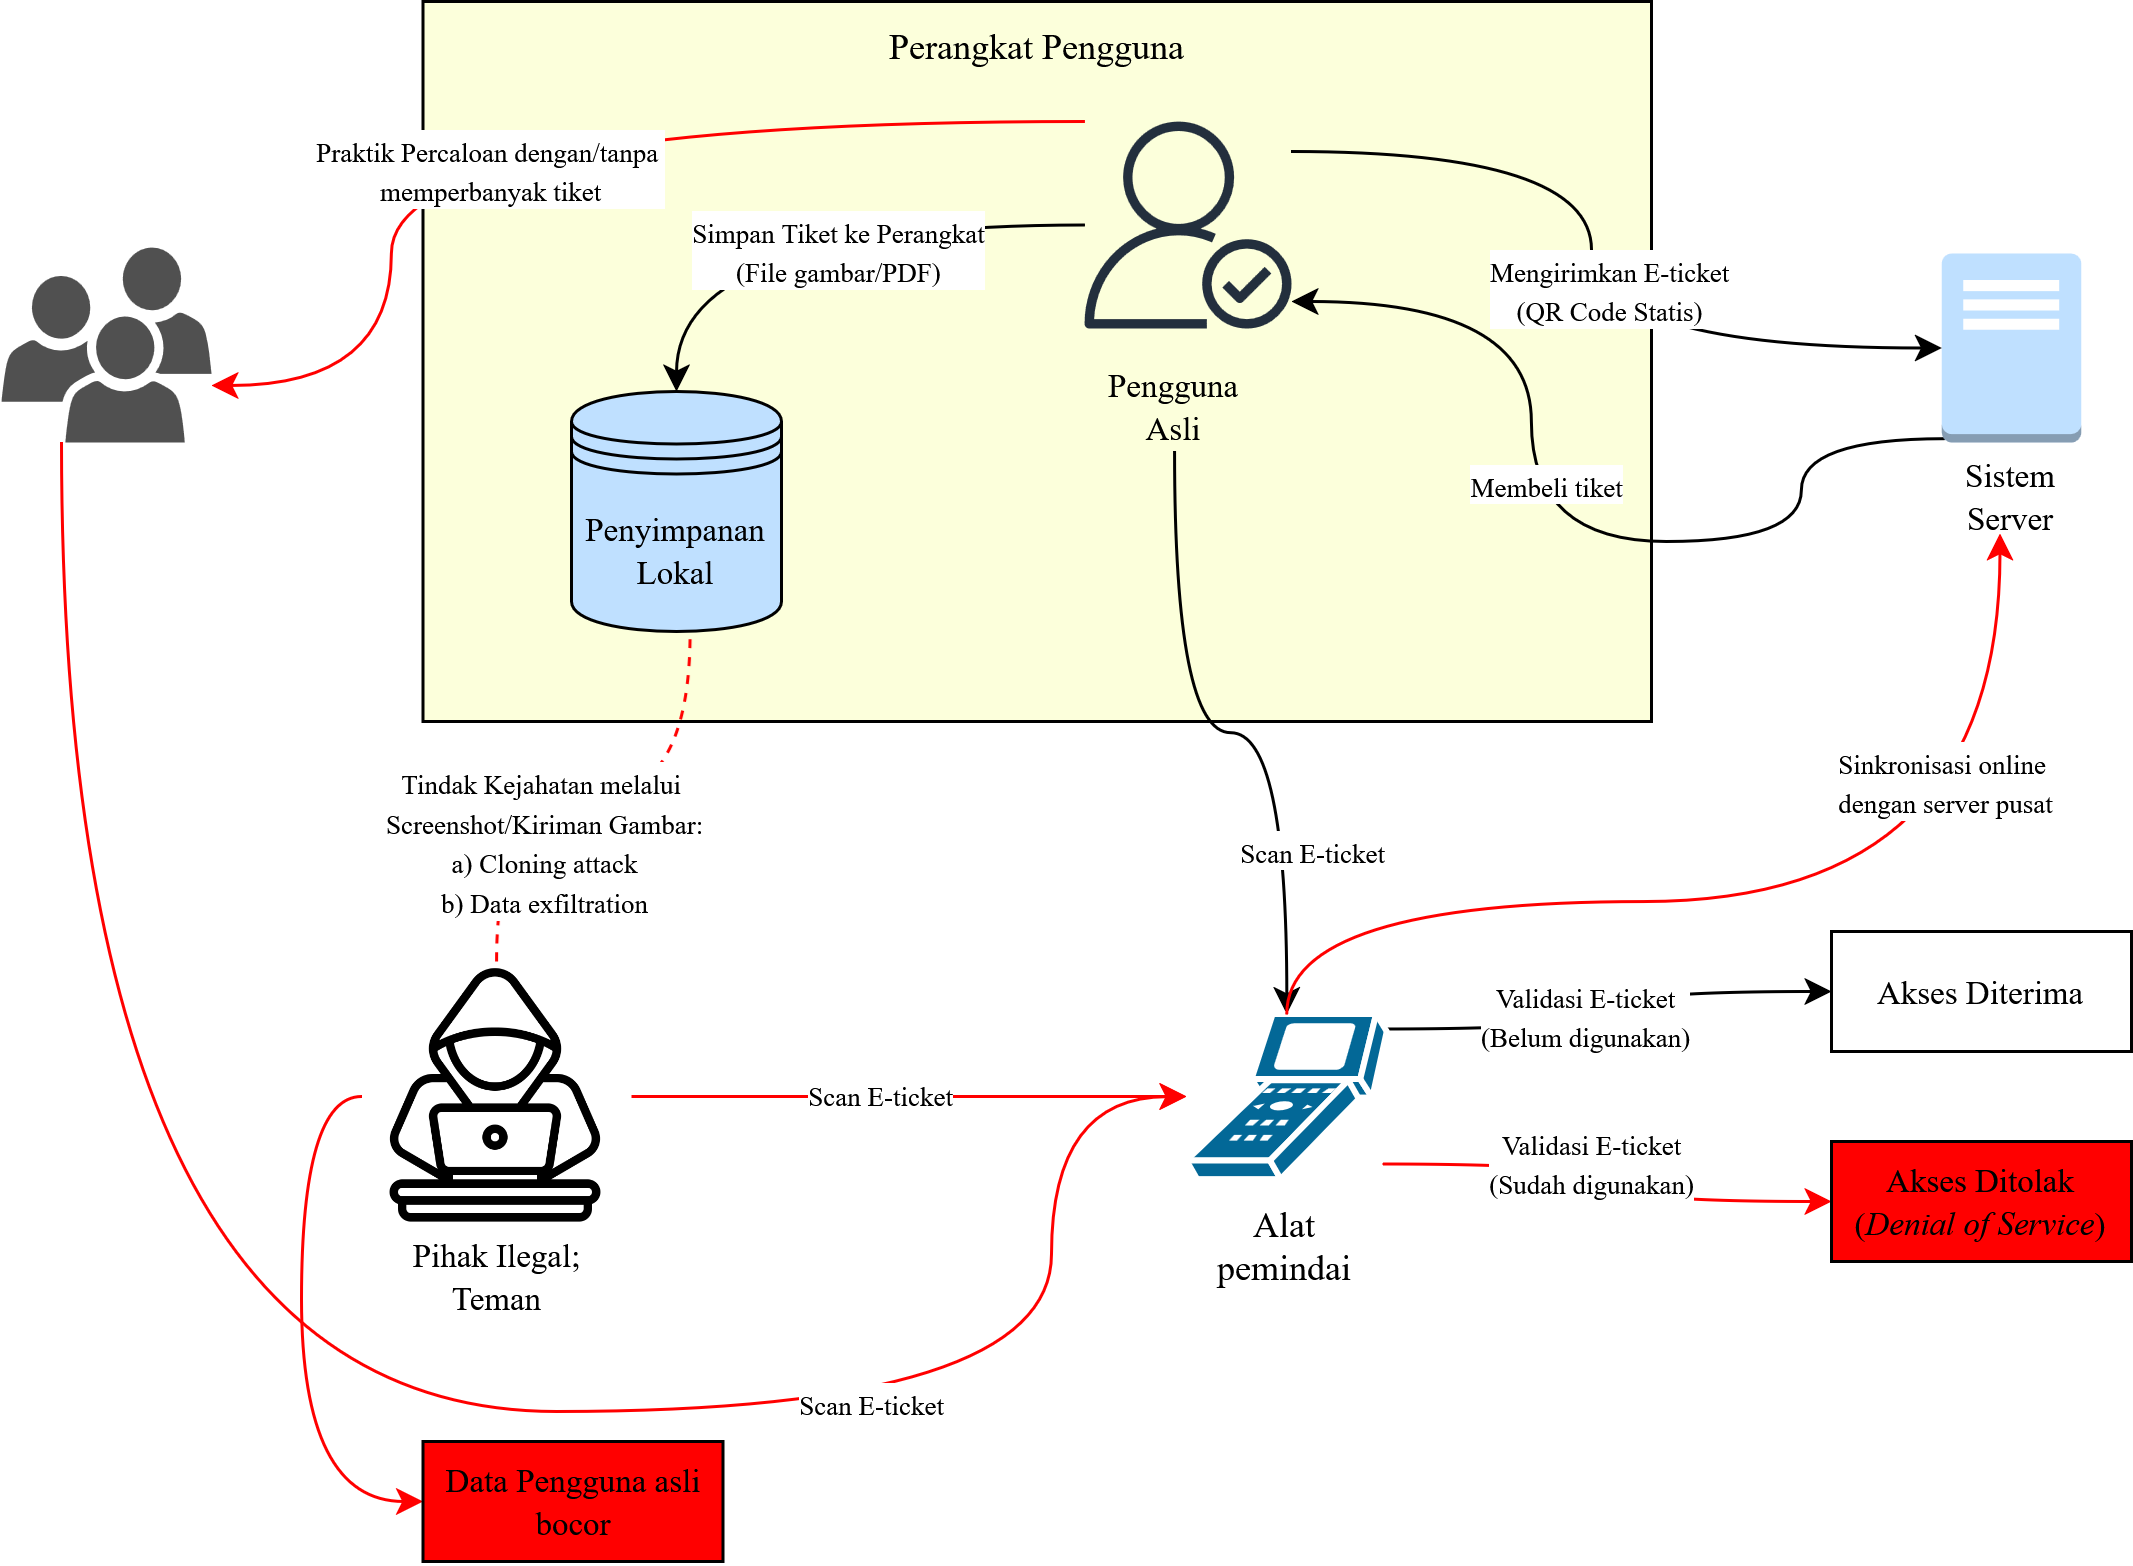
\includegraphics[width=\textwidth, keepaspectratio]{images/TA-model_konseptual.png}
    \caption{Model Konseptual dan Titik Kerentanan Sistem \textit{E-Ticket} Konvensional}
    \label{fig:current_system_flow}
\end{figure}

Sebagaimana diilustrasikan pada Gambar \ref{fig:current_system_flow}, proses dimulai ketika pengguna asli membeli tiket dari sistem peladen. Tiket yang dibangkitkan kemudian dikirim dan disimpan ke dalam penyimpanan lokal perangkat pengguna dalam format berkas statis (seperti citra matriks kode QR atau berkas PDF). Sifat data yang statis dan tersimpan secara lokal ini menciptakan celah keamanan yang digambarkan melalui vektor ancaman utama pada diagram:

\begin{enumerate}
    \item \textbf{Distribusi Tiket Tidak Terkendali (Praktik Percaloan):} 
    Seperti terlihat pada alur panah bagian atas diagram, ketiadaan mekanisme validasi berbasis waktu (\textit{time-based validation}) memungkinkan pengguna asli untuk mendistribusikan satu tiket kepada banyak pihak lain hanya dengan menyalin citra kode QR. Karena kode tersebut berlaku tanpa batas waktu hingga dipindai (statis), tiket dapat digandakan dan dijual kembali dengan mudah tanpa terikat pada sesi aplikasi pengguna yang sah. Hal ini menyuburkan praktik percaloan, yaitu ketika tiket dijual dengan harga yang melambung tinggi tanpa kendali penyelenggara resmi sehingga merusak ekosistem penjualan tiket yang sehat.
    
    \item \textbf{Ancaman Penggandaan (\textit{Cloning Attack}) dan Penolakan Layanan:} 
    Celah pada penyimpanan lokal memungkinkan pihak ilegal mengambil alih tiket melalui tangkapan layar (\textit{screenshot}). Hal ini menciptakan kondisi balapan (\textit{race condition}) antarpemegang tiket yang identik saat proses verifikasi di pintu masuk. Sebagaimana ditunjukkan pada alur validasi diagram, jika pihak ilegal berhasil memindai tiket lebih awal, maka alat pemindai akan mencatat tiket sebagai ``Sudah Digunakan''. Akibatnya, pengguna asli yang datang belakangan akan mengalami penolakan akses (\textit{Denial of Service}), meskipun memiliki bukti pembayaran yang sah.
    
    \item \textbf{Kebocoran Data Pribadi (\textit{Data Exfiltration}):} 
    Penyimpanan tiket statis tanpa perlindungan memadai pada memori lokal membuka peluang terjadinya eksfiltrasi data. Informasi sensitif pengguna yang melekat pada tiket (seperti nama, nomor identitas kependudukan, atau detail pesanan) dapat dengan mudah terbaca apabila dokumen tiket digital tersebut jatuh ke tangan pihak tidak bertanggung jawab, sebagaimana digambarkan pada blok ``Data Pengguna Asli Bocor''.

    \item \textbf{Ketergantungan Konektivitas (\textit{Single Point of Failure}):}
    Sebagaimana ditunjukkan oleh garis alur ``Sinkronisasi online dengan server pusat'', mekanisme validasi saat ini mewajibkan alat pemindai untuk terus terhubung ke peladen guna memverifikasi status tiket. Hal ini menciptakan risiko Titik Kegagalan Tunggal (\textit{Single Point of Failure}). Apabila terjadi gangguan infrastruktur jaringan di lokasi acara atau kelebihan beban akibat saturasi trafik seluler ribuan pengunjung, proses validasi akan terhenti total. Kondisi ini memicu penumpukan antrean massal yang parah di pintu gerbang dan melumpuhkan operasional acara.

    \item \textbf{Celah Serangan Multi-Gerbang Luring dan Relai Jarak Jauh (\textit{Multi-Gate Offline Replay \& Relay}):}
    Untuk mengatasi ketergantungan koneksi internet, beberapa pendekatan mencoba beralih ke mekanisme luring (\textit{offline}) yang dikombinasikan dengan kode dinamis berbasis waktu (seperti algoritma TOTP standar). Namun, analisis menunjukkan bahwa langkah ini melahirkan celah baru yang fatal pada acara dengan banyak gerbang masuk (\textit{multi-gate}). Karena algoritma TOTP standar hanya terikat pada parameter waktu universal dan pemindai beroperasi tanpa sinkronisasi waktu nyata (\textit{real-time}) antar-gerbang, sebuah tiket yang digandakan dapat dipindai secara simultan pada dua gerbang berbeda dalam jendela waktu aktif yang sama. Selain itu, tiket dinamis tetap rentan terhadap serangan relai jarak jauh (\textit{remote relay attack}), di mana seorang penipu menyiarkan citra kode QR dinamis yang sedang aktif kepada rekannya melalui panggilan video (\textit{video call}) atau tangkapan layar instan. 

    Salah satu alternatif awal yang dipertimbangkan untuk mengikat lokasi pemindaian adalah pemanfaatan koordinat satelit (\textit{GPS Geofencing}). Namun, pendekatan ini memiliki kelemahan signifikan di lapangan [Perlu Sitasi: Jurnal analisis akurasi dan kerentanan GPS spoofing pada aplikasi seluler]: (1) akurasi sinyal GPS menurun drastis pada area dalam ruangan (\textit{indoor}), stadion beratap kanopi beton, atau di tengah kepadatan kerumunan massal (\textit{multipath fading}), sehingga tidak mampu membedakan gerbang-gerbang masuk yang bersebelahan dengan jarak beberapa meter, dan (2) koordinat GPS sangat mudah dimanipulasi melalui aplikasi lokasi palsu (\textit{Mock Location / Fake GPS}) pada perangkat seluler. Keterbatasan ini menegaskan pentingnya mekanisme validasi berbasis proksimitas fisik jarak dekat yang kebal manipulasi peranti lunak, seperti teknologi \textit{Bluetooth Low Energy} (BLE).
\end{enumerate}

Kondisi-kondisi di atas menegaskan bahwa arsitektur pertiketan konvensional belum memenuhi prinsip keamanan informasi (\textit{Confidentiality, Integrity, Availability}) yang memadai untuk menangani kontrol akses bernilai tinggi.

\section{Analisis Kebutuhan}
\label{sec:analisis_kebutuhan}

Tahap analisis kebutuhan bertujuan untuk mendefinisikan spesifikasi sistem yang harus dipenuhi guna mengatasi permasalahan yang telah diidentifikasi pada model sistem saat ini. Sesuai metodologi rekayasa perangkat lunak menurut \textcite{pressman2019}, analisis ini dibagi menjadi identifikasi masalah pemangku kepentingan, kebutuhan fungsional, dan kebutuhan non-fungsional.

\subsection{Identifikasi Masalah Pengguna dan Penyelenggara}
\label{subsec:identifikasi_masalah}
Berdasarkan analisis kondisi saat ini, terdapat lima permasalahan kritis yang dihadapi oleh pemangku kepentingan utama, yaitu penyelenggara acara (\textit{event organizer}) dan pengguna (pemegang tiket yang sah):

\begin{enumerate}
    \item \textbf{Distribusi Tiket Tidak Terkendali:} Sifat statis dari visualisasi kode QR membuat informasi validitas tiket melekat permanen pada citra tanpa batasan waktu tayang. Akibatnya, sistem tidak dapat membedakan antara pemegang tiket asli yang mengakses melalui aplikasi resmi dengan pihak lain yang hanya bermodalkan salinan gambar, menyuburkan praktik percaloan dan penipuan tiket sekunder.
    
    \item \textbf{Penolakan Layanan akibat Penggandaan (\textit{Race Condition}):} Pemegang tiket yang sah berisiko gagal memasuki area acara jika tiket mereka telah digandakan (\textit{cloning}) dan dipindai lebih dulu oleh pihak ilegal. Kondisi ini menciptakan persaingan di pintu masuk; siapa yang memindai lebih dulu akan diterima, sedangkan pengguna sah yang datang belakangan akan tertolak sistem karena tiket berstatus sudah digunakan.
    
    \item \textbf{Kerentanan Privasi Data Pribadi:} Informasi identitas pribadi pengguna (seperti NIK, nama lengkap, dan nomor kontak) kerap disertakan langsung ke dalam muatan kode QR dalam format teks terbuka (\textit{plaintext}). Ketiadaan perlindungan privasi berbasis desain (\textit{Privacy by Design}) membuka peluang terjadinya eksfiltrasi data oleh pihak ketiga yang memindai kode QR secara tidak sah.
    
    \item \textbf{Ketergantungan Koneksi Internet dan Titik Kegagalan Tunggal:} Ketergantungan absolut pada kueri basis data pusat secara \textit{online} saat pemindaian menyebabkan proses validasi rentan lumpuh total ketika terjadi gangguan jaringan seluler di lokasi acara, memicu kekacauan antrean di pintu masuk.

    \item \textbf{Kerentanan Multi-Gerbang Luring dan Serangan Relai Jarak Jauh:} Penyelenggara acara berskala besar menghadapi risiko pembobolan gerbang ganda saat beroperasi secara luring, di mana pembatasan berbasis waktu saja tidak mampu membedakan apakah pengguna benar-benar hadir secara fisik di gerbang tertentu. Ketiadaan pengikatan spasial memungkinkan tiket dinamis direlai atau dibagikan secara instan melalui siaran layar (\textit{screen sharing}) ke pihak lain di luar lokasi.
\end{enumerate}

\subsection{Kebutuhan Fungsional}
\label{subsec:kebutuhan_fungsional}
Kebutuhan fungsional mendefinisikan kapabilitas dan fitur spesifik yang harus disediakan oleh perangkat lunak untuk menjawab permasalahan di atas. Rincian kebutuhan fungsional sistem \textit{Dynamic Secure QR Code} dijabarkan pada Tabel \ref{tab:functional_req}.

\begin{longtable}{|l|p{4.5cm}|p{7.5cm}|}
    \caption{Daftar Kebutuhan Fungsional Sistem}\label{tab:functional_req} \\
    \hline
    \textbf{Kode} & \textbf{Kebutuhan Fungsional} & \textbf{Deskripsi} \\
    \hline
    \endfirsthead
    
    \caption[]{Daftar Kebutuhan Fungsional Sistem (lanjutan)} \\
    \hline
    \textbf{Kode} & \textbf{Kebutuhan Fungsional} & \textbf{Deskripsi} \\
    \hline
    \endhead
    
    \hline
    \multicolumn{3}{r}{\textit{Bersambung ke halaman berikutnya}} \\
    \endfoot
    
    \hline
    \endlastfoot
    
    FR-01 & Penerbitan \textit{E-ticket} & Sistem (Peladen) dapat menerbitkan tiket elektronik baru yang memuat atribut tiket non-sensitif, kunci rahasia spesifik pengguna (\textit{user secret key}), dan tanda tangan digital, lalu mendistribusikannya secara aman ke perangkat pengguna. \\
    \hline
    FR-02 & Pembangkitan Kode QR Dinamis \textit{Gate-Bound} & Sistem (Aplikasi Pengguna) dapat memvisualisasikan tiket dalam bentuk kode QR dinamis yang diperbarui otomatis setiap interval waktu tertentu (30 detik) berdasarkan kombinasi token waktu (TOTP) dan pengenal gerbang ($Gate\_ID$). \\
    \hline
    FR-03 & Minimalisasi Data \& Privasi & Sistem menerapkan prinsip \textit{Data Minimization} dengan membatasi muatan data kode QR hanya pada atribut teknis non-sensitif, sehingga data pribadi pengguna (PII) tidak terekspos dalam kode QR. \\
    \hline
    FR-04 & Integritas Data Tiket & Sistem menyertakan mekanisme penandatanganan digital berbasis ECDSA pada data tiket untuk menjamin keaslian penerbit dan memastikan informasi tidak dimodifikasi oleh pihak ketiga. \\
    \hline
    FR-05 & Verifikasi Lokal \textit{Stateless} & Aplikasi pemindai dapat memverifikasi tanda tangan digital dan validitas token TOTP secara mandiri (\textit{offline}) menggunakan skema derivasi kunci KDF tanpa membutuhkan sambungan internet ke peladen pusat. \\
    \hline
    FR-06 & Validasi Token Waktu & Aplikasi pemindai dapat memvalidasi keabsahan token dinamis pengguna dengan menyertakan toleransi pergeseran waktu jam (\textit{clock drift}) sebesar $\pm 1$ langkah waktu. \\
    \hline
    FR-07 & Manajemen \textit{Cache} Lokal & Aplikasi pemindai memiliki basis data lokal (\textit{Local Cache}) untuk mencatat tiket yang telah lolos verifikasi guna mencegah serangan penggunaan ganda (\textit{replay/cloning}) secara instan di gerbang fisik. \\
    \hline
    FR-08 & Sinkronisasi Asinkron (\textit{Batching}) & Aplikasi pemindai mendukung pengiriman data log kehadiran secara berkala (\textit{batching}) ke peladen pusat di latar belakang ketika koneksi internet tersedia untuk rekonsiliasi data akhir. \\
    \hline
    FR-09 & Penyiaran dan Deteksi Sinyal BLE & Perangkat pemindai gerbang dapat menyiarkan identitas gerbang ($Gate\_ID$) melalui sinyal BLE \textit{beacon}, dan aplikasi pengguna dapat mendeteksi sinyal proksimitas tersebut dalam radius tertentu untuk mengaktifkan kode akses dinamis. \\
    \hline

\end{longtable}

\subsection{Kebutuhan Non-fungsional}
\label{subsec:kebutuhan_nonfungsional}
Kebutuhan non-fungsional mendefinisikan atribut kualitas, batasan operasional, dan kriteria kinerja yang harus dipenuhi oleh sistem. Rincian kebutuhan non-fungsional dijabarkan pada Tabel \ref{tab:non_functional_req}.

\begin{longtable}{|l|p{4.5cm}|p{7.5cm}|}
    \caption{Daftar Kebutuhan Non-fungsional Sistem}\label{tab:non_functional_req} \\
    \hline
    \textbf{Kode} & \textbf{Parameter} & \textbf{Deskripsi} \\
    \hline
    \endfirsthead
    
    \caption[]{Daftar Kebutuhan Non-fungsional Sistem (lanjutan)} \\
    \hline
    \textbf{Kode} & \textbf{Parameter} & \textbf{Deskripsi} \\
    \hline
    \endhead
    
    \hline
    \multicolumn{3}{r}{\textit{Bersambung ke halaman berikutnya}} \\
    \endfoot
    
    \hline
    \endlastfoot

    NFR-01 & Keamanan (\textit{Security}) & Sistem harus menerapkan Tanda Tangan Digital ECDSA untuk integritas data dan prinsip \textit{Privacy by Design} untuk kerahasiaan identitas, serta memastikan ketahanan terhadap upaya pemalsuan dan penggandaan tiket. \\
    \hline
    NFR-02 & Kinerja (\textit{Performance}) & Proses pembangkitan kode QR di sisi pengguna dan proses verifikasi kriptografi di sisi pemindai harus dapat diselesaikan dalam waktu kurang dari 2 detik (latensi rendah) untuk mencegah antrean. \\
    \hline
    NFR-03 & Ketersediaan (\textit{Availability}) & Fitur validasi tiket utama harus memiliki tingkat ketersediaan tinggi dan tetap berfungsi penuh dalam mode luring (\textit{offline}) tanpa ketergantungan koneksi jaringan internet aktif. \\
    \hline
    NFR-04 & Kompatibilitas (\textit{Compatibility}) & Sistem harus dapat dioperasikan pada perangkat seluler bersistem operasi Android umum dan tidak mensyaratkan perangkat keras tambahan selain kamera dan modul Bluetooth standar. \\
    \hline
    NFR-05 & Validasi Spasial (\textit{Proximity}) & Sistem harus mampu membatasi keabsahan token dinamis hanya dalam radius deteksi fisik operasional gerbang masuk (berdasarkan ambang batas daya terima sinyal $RSSI \ge -75\text{ dBm}$) guna memitigasi serangan relai jarak jauh. \\
    \hline
    
\end{longtable} 

\section{Analisis Pemilihan Solusi}
\label{sec:pemilihan_solusi}

Berdasarkan identifikasi masalah yang kompleks, yaitu tuntutan keamanan tinggi (anti-pemalsuan dan anti-penggandaan) yang berbenturan dengan tuntutan operasional lapangan (ketersediaan layanan saat jaringan internet padat atau terputus), diperlukan analisis mendalam untuk menentukan pendekatan solusi terbaik. Bagian ini menguraikan sepuluh alternatif solusi yang mungkin diterapkan—mulai dari prosedur manual, pendekatan berbasis perangkat keras, pemanfaatan satelit GPS, hingga solusi kriptografi terdesentralisasi—kemudian mengevaluasinya secara terukur menggunakan parameter yang diturunkan dari kebutuhan non-fungsional.

\subsection{Alternatif Solusi}
\label{subsec:alternatif_solusi}
Terdapat sepuluh kandidat solusi yang diidentifikasi dapat menjawab sebagian atau seluruh permasalahan sistem pertiketan:

\begin{enumerate}
    \item \textbf{Alt-01: Validasi Visual Tambahan (\textit{Watermarking} / Animasi):} Menambahkan elemen visual bergerak (seperti animasi GIF atau penanda warna dinamis) pada desain tiket aplikasi agar petugas dapat mengenali keasliannya secara kasat mata. Meskipun biaya implementasi rendah, metode ini tidak efektif menahan manipulasi modern berupa rekaman layar (\textit{screen recording}), serta bergantung sepenuhnya pada ketelitian mata petugas (\textit{human error}) yang memperlambat laju antrean di gerbang masuk.
    
    \item \textbf{Alt-02: Pencocokan Identitas Fisik Manual (KTP/ID):} Mewajibkan pengunjung memperlihatkan kartu identitas fisik asli (seperti KTP atau paspor) untuk dicocokkan dengan nama pada tiket dan wajah pengunjung oleh petugas gerbang. Pendekatan ini efektif mematikan praktik percaloan tiket, namun menimbulkan inefisiensi operasional yang luar biasa parah berupa penumpukan antrean panjang (\textit{bottleneck}) karena durasi verifikasi manual memakan waktu hingga puluhan detik per orang.
    
    \item \textbf{Alt-03: Integrasi Ekosistem Aplikasi Tertutup (\textit{E-Wallet} / \textit{M-Banking}):} Mengunci tiket secara internal di dalam aplikasi perbankan atau dompet digital tertentu sehingga tidak dapat diekspor. Solusi ini mengurangi pemindahtanganan liar, namun membatasi inklusivitas pengguna secara sepihak (\textit{vendor lock-in}), serta tetap mewajibkan konektivitas internet aktif saat memuat halaman tiket di pintu masuk.
    
    \item \textbf{Alt-04: Autentikasi Biometrik (Pengenalan Wajah / Sidik Jari):} Menggantikan tiket fisik/digital sepenuhnya dengan memindai wajah atau sidik jari pengunjung di gerbang masuk. Tingkat keamanan dan kepraktisan sangat tinggi, namun membutuhkan investasi infrastruktur pemindai biometrik yang sangat mahal, menimbulkan resistensi privasi data (\textit{biometric privacy risks}), serta rentan mengalami kelumpuhan total jika pangkalan data biometrik pusat terputus koneksinya.
    
    \item \textbf{Alt-05: Tiket Berbasis \textit{Blockchain} / NFT (\textit{Smart Contract}):} Memanfaatkan teknologi buku besar terdistribusi (\textit{blockchain}) untuk melacak riwayat kepemilikan tiket dan membatasi transaksi pasar sekunder melalui kontrak pintar. Secara logis pendekatan ini menertibkan distribusi tiket, namun implementasinya di lapangan tidak praktis, memerlukan biaya transaksi (\textit{gas fee}), dan mewajibkan konektivitas internet \textit{real-time} untuk kueri status blok yang tidak realistis pada kondisi kerumunan massal.
    
    \item \textbf{Alt-06: Verifikasi Sandi Sekali Pakai Seluler (SMS / WhatsApp OTP):} Mengharuskan pengguna meminta kode OTP melalui jaringan telekomunikasi seluler saat tiba di gerbang masuk sebelum tiket dapat dibuka. Metode ini memiliki risiko ketersediaan paling kritis karena spektrum frekuensi seluler operator hampir selalu tersaturasi (\textit{network congestion}) di lokasi acara besar, mengakibatkan latensi pengiriman SMS yang sangat tinggi atau bahkan gagal terkirim sama sekali.
    
    \item \textbf{Alt-07: Validasi Berbasis Perangkat Keras Radio (NFC / RFID Tap):} Menyimpan tiket dalam elemen aman (\textit{Secure Element}) ponsel cerdas dan divalidasi dengan menempelkan perangkat ke pembaca gerbang (\textit{tap-to-enter}). Proses pemindaian sangat cepat (kurang dari 0,5 detik) dan kebal terhadap tangkapan layar. Namun, solusi ini terkendala aspek kompatibilitas karena sebagian besar ponsel cerdas kelas menengah ke bawah di Indonesia belum dilengkapi sensor NFC, sehingga berpotensi mengecualikan banyak calon penonton.
    
    \item \textbf{Alt-08: Kode QR Dinamis Terpusat (\textit{Online Token API}):} Aplikasi pengguna meminta kode QR baru yang berlaku singkat (misal 10 detik) ke peladen pusat secara berkala melalui panggilan API. Solusi ini efektif menggagalkan tangkapan layar statis, namun menciptakan ketergantungan mutlak pada ketersediaan internet (\textit{Single Point of Failure}). Apabila jaringan internet di gerbang terputus, tiket tidak dapat dimuat atau divalidasi, memicu penumpukan antrean massal. Selain itu, solusi ini tidak dapat mencegah penyerang yang melakukan siaran langsung (\textit{live stream}) kode QR kepada rekannya di gerbang.
    
    \item \textbf{Alt-09: Pembatasan Geografis Berbasis Satelit (\textit{GPS Geofencing}):} Mengintegrasikan koordinat GPS perangkat pengguna ke dalam validasi tiket untuk memastikan bahwa pengguna benar-benar berada di area acara sebelum tiket dinamis diaktifkan. Meskipun didukung oleh hampir seluruh ponsel cerdas, pendekatan ini memiliki kelemahan mendasar: (1) akurasi GPS menurun drastis di area dalam ruangan atau terhalang atap kanopi gerbang sehingga tidak mampu membedakan antar-gerbang fisik yang berjarak dekat, (2) koordinat GPS sangat rentan dimanipulasi menggunakan peranti lunak lokasi palsu (\textit{Fake GPS / Mock Location}) di ponsel pintar, dan (3) proses penentuan posisi satelit membutuhkan waktu (\textit{locking latency}) serta menguras daya baterai.
    
    \item \textbf{Alt-10: Kode QR Dinamis Hibrida dengan BLE (Solusi Tugas Akhir):} Solusi yang diusulkan menggabungkan komputasi kriptografi di sisi klien (\textit{client-side processing}) dan pembatasan spasial berbantuan nirkabel gelombang radio lokal. Sistem menggunakan algoritma TOTP untuk menyegarkan kode QR secara berkala dan Tanda Tangan Digital (ECDSA) untuk integritas data tanpa bergantung pada peladen. Pemanfaatan sinyal \textit{Bluetooth Low Energy} (BLE) \textit{beacon} pada gerbang berfungsi sebagai pengikat spasial (\textit{Gate-Bound}): aplikasi ponsel harus menangkap sinyal fisik gerbang lokal ($Gate\_ID$) untuk membangkitkan token TOTP yang valid. Pendekatan ini mematikan celah penggandaan tangkapan layar, kebal serangan relai jarak jauh, menjamin ketersediaan luring penuh (\textit{offline-first}), serta kompatibel dengan perangkat seluler umum.
\end{enumerate}

\subsection{Analisis Penentuan Solusi}
\label{subsec:penentuan_solusi}
Untuk menentukan solusi yang paling optimal secara objektif, kesepuluh alternatif dievaluasi menggunakan lima kriteria evaluasi yang diturunkan langsung dari kebutuhan non-fungsional sistem:
\begin{enumerate}
    \item \textbf{Keamanan (\textit{Security}):} Kemampuan sistem menggagalkan pemalsuan, penggandaan (\textit{cloning}), manipulasi data, dan eksfiltrasi identitas pribadi (merujuk pada NFR-01).
    \item \textbf{Kinerja (\textit{Performance}):} Kecepatan dan kelancaran proses pemindaian per pengunjung (latensi di bawah 2 detik) guna mengurai antrean gerbang masuk (merujuk pada NFR-02).
    \item \textbf{Ketersediaan Luring (\textit{Availability}):} Kemampuan sistem beroperasi secara penuh dan mandiri dalam kondisi jaringan internet terputus total (merujuk pada NFR-03).
    \item \textbf{Kompatibilitas (\textit{Compatibility}):} Aksesibilitas bagi mayoritas perangkat seluler pengguna tanpa mewajibkan peranti keras eksklusif seperti sensor NFC (merujuk pada NFR-04).
    \item \textbf{Validasi Spasial (\textit{Proximity}):} Kemampuan sistem mengonfirmasi kehadiran fisik pengguna di lokasi gerbang spesifik guna menolak penyerangan relai jarak jauh dan pembobolan multi-gerbang luring (merujuk pada NFR-05).
\end{enumerate}

Perbandingan performa dari setiap alternatif solusi terhadap kelima kriteria evaluasi disajikan dalam Matriks Keputusan pada Tabel \ref{tab:decision_matrix}.

\begin{table}[htbp]
    \caption{Matriks Keputusan Pemilihan Solusi Sistem \textit{E-Ticket}}
    \label{tab:decision_matrix}
    \centering
    \begin{tabularx}{\textwidth}{ c >{\raggedright\arraybackslash}X c c c c c }
        \toprule
        \textbf{ID} & \textbf{Alternatif Solusi} & \textbf{Keamanan} & \textbf{Ketersediaan} & \textbf{Kompatibilitas} & \textbf{Kinerja} & \textbf{Spasial} \\
        \midrule
        01 & Visual (\textit{Watermarking}) & Buruk & Sangat Baik & Sangat Baik & Buruk & Buruk \\
        02 & Pencocokan KTP/ID Manual & Sangat Baik & Sangat Baik & Sangat Baik & Sangat Buruk & Sangat Baik \\
        03 & Integrasi \textit{E-Wallet} & Baik & Buruk & Buruk & Sedang & Buruk \\
        04 & Biometrik Wajah/Sidik Jari & Sangat Baik & Buruk & Sedang & Baik & Sangat Baik \\
        05 & Tiket \textit{Blockchain} / NFT & Baik & Buruk & Baik & Sedang & Buruk \\
        06 & SMS/WhatsApp OTP & Sedang & Sangat Buruk & Sangat Baik & Buruk & Buruk \\
        07 & Validasi Perangkat Keras NFC & Sangat Baik & Sangat Baik & Buruk & Sangat Baik & Sangat Baik \\
        08 & QR Dinamis Terpusat (\textit{Online}) & Baik & Sangat Buruk & Baik & Sedang & Buruk \\
        09 & Pembatasan Satelit GPS & Buruk & Sedang & Sangat Baik & Sedang & Buruk \\
        \midrule
        \textbf{10} & \textbf{QR Hibrida + BLE (Usulan)} & \textbf{Sangat Baik} & \textbf{Sangat Baik} & \textbf{Baik} & \textbf{Sangat Baik} & \textbf{Sangat Baik} \\
        \bottomrule
    \end{tabularx}
\end{table}

Berdasarkan analisis komparatif pada Tabel \ref{tab:decision_matrix}, penelitian ini memutuskan untuk mengadopsi \textbf{Alt-10 (Kode QR Dinamis Hibrida dengan BLE)}. 

Justifikasi ilmiah pemilihan ini didasarkan pada eliminasi kelemahan alternatif-alternatif lainnya:
\begin{enumerate}[a)]
    \item Solusi manual seperti pencocokan KTP (Alt-02) gugur karena kinerja yang sangat lambat dan memicu kemacetan antrean parah di gerbang masuk.
    \item Seluruh solusi berbasis daring (Alt-03, Alt-05, Alt-06, dan Alt-08) memiliki titik kegagalan tunggal (\textit{Single Point of Failure}) pada parameter Ketersediaan Luring, sehingga sangat berisiko melumpuhkan operasional saat jaringan seluler di lokasi acara mengalami saturasi trafik.
    \item Solusi berbasis perangkat keras eksklusif seperti NFC (Alt-07) memiliki kendala serius pada aspek Kompatibilitas perangkat di Indonesia, sehingga kurang inklusif bagi pengguna ponsel cerdas kelas menengah ke bawah.
    \item Solusi berbasis satelit GPS (Alt-09) gugur pada parameter Keamanan dan Validasi Spasial karena rentan terhadap manipulasi lokasi palsu (\textit{mock location}) serta memiliki resolusi jarak yang terlalu lebar sehingga tidak dapat mengisolasi pintu gerbang individual.
\end{enumerate}

Dengan demikian, penggabungan algoritma TOTP, Tanda Tangan Digital ECDSA, dan pengikatan spasial proksimitas jarak dekat berbasis BLE (\textbf{Alt-10}) merupakan satu-satunya pendekatan yang mampu memuaskan kelima kriteria kebutuhan secara optimal, menjadikannya fondasi perancangan sistem yang dikembangkan pada Bab IV.